%%%%%%%%%%%%%%%%%%%%%%%%%%%%%%%%%%%%%%%%%%%%%%%%%%%%%%%%%
% LaTeX Beamer Presentation
%
% Theme: Madrid (as requested)
%
% FIX: Implemented automatic Table of Contents display at the 
%      beginning of each defined section using \AtBeginSection.
%%%%%%%%%%%%%%%%%%%%%%%%%%%%%%%%%%%%%%%%%%%%%%%%%%%%%%%%%

\documentclass{beamer}

\mode<presentation>
{
  % --- THEME: Using the robust Madrid theme as requested. ---
  \usetheme{Madrid}
  
  % --- TEMPLATE SETTINGS ---
  \setbeamertemplate{navigation symbols}{} % Hides navigation buttons
  % Now uses the Madrid default footline.


}

% Setting Logo in every slide
\logo{
\includegraphics[width=.1\textwidth]{../figures/AIIIMA.jpeg}}
% --- Setting the acronyms
\usepackage[nolist]{acronym}
\begin{acronym}
  \acro{BC}[BC]{Breast Cancer}
  \acro{MG}[MG]{Mammography}
  \acro{TG}[TG]{Thermography}
  \acro{CAD}[CAD]{computer-aided detection}
  \acro{CNNs}[CNNs]{convolutional neural networks}
  \acro{ViTs}[ViTs]{Vision Transformers}
  \acro{ViT}[ViT]{Vision Transformer}
  \acro{FDA}[FDA]{Food and Drug Administration}
  \acro{SIT}[SIT]{Static Infrared Thermography}
  \acro{DIT}[DIT]{Dynamic Infrared Thermography}
  \acro{SLR}[SLR]{Systematic Literature Review}
  \acro{PICOC}[PICOC]{Population, Intervention, Comparison, Outcome,
    Context}
  \acro{DL}[DL]{Deep Learning}
  \acro{AI}[AI]{Artificial Intelligence}
  \acro{NLP}[NLP]{Natural Language Processing}
  \acro{TCN}[TCN]{Temporal Convolutional Network}
  \acro{TDL}[TDL]{Time Distributed Layers}
  \acro{RNN}[RNN]{Recurrent Neural Networks}
  \acro{HAR}[HAR]{Human Activity Recognition}
  \acro{ViViTs}[ViViTs]{Video Vision Transformers}
  \acro{ViViT}[ViViT]{Video Vision Transformer}
  \acro{IR}[IR]{Infrared}
  \acro{TM}[TM]{Temperature Maps}
  \acro{LSTM}[LSTM]{Long Short Memory}
  \acro{UFF}[UFF]{Universidade Federal Fluminense}
  \acro{AUC}[AUC]{Area Under the Receiver Operating Characteristic
    Curve}
  \acro{lr}[lr]{learning rate}
  \acro{TL}[TL]{Transfer Learning}
  \acro{FT}[FT]{Fine Tuning}
\end{acronym}


% --- AUTOMATIC TOC AT BEGINNING OF EACH SECTION ---
\AtBeginSection[]
{
  \begin{frame}
    \frametitle{Presentation Outline}
    \tableofcontents[currentsection] % Only shows the current section/subsection list
  \end{frame}
}

% --- PACKAGES ---
\usepackage[utf8]{inputenc}
\usepackage{graphicx}      % For images
\usepackage{booktabs}      % For professional tables
\usepackage{amsmath}       % For math
\usepackage{amssymb}       % For math
\usepackage{xcolor}        % Keeping xcolor for the custom teal color
% in the bar chart
\usepackage{array}           % For extended table functionality
\usepackage{tabularx}
\usepackage{multirow}        % For multirow cells
\usepackage[autolanguage]{numprint}
\usepackage[style=ieee,backend=biber]{biblatex}
\addbibresource{../bibliography.bib} % your .bib file


\definecolor{myteal}{RGB}{17, 202, 160} % Keeping only the necessary color definition

% --- PRESENTATION METADATA ---
\title[Video Transformers for Dynamic IR in BC]{
  Video Transformers for Dynamic Breast Infrared
  Imaging Classification
}
\author[Falconi, et al.]{
  Lenin G. Falconi \inst{1} \and
  Maria Pérez \inst{1} \and
  Marco E. Benalcázar \inst{1} \and \\
  Aura Conci \inst{2}
}
\institute[EPN \and UFF]{
  \inst{1} Escuela Politécnica Nacional, Quito, Ecuador \\
  \inst{2} Instituto de Computação, Universidade Federal Fluminense, Brazil
}
\date[AIIIMA 2025]{4th International Conference on AIIIMA 2025}

% --- DOCUMENT START ---
\begin{document}

% \titlegraphic{
%   
\includegraphics[width=1.5cm]{../figures/AIIIMA.jpeg}
% }

% --- SLIDE 1: TITLE PAGE ---
\begin{frame}
  \titlepage
\end{frame}

% Table of Contents
\begin{frame}
    \frametitle{Overview}
    \tableofcontents
\end{frame}
% ===================================
% SECTION 1: INTRODUCTION
% ===================================
\section{Introduction}

% --- SLIDE 2: THE CHALLENGE ---

\subsection{Breast Cancer}

\begin{frame}
  \frametitle{The Challenge of Early Detection}
  \begin{columns}[T]
    % Column 1
    \begin{column}{0.48\textwidth}
      \begin{block}{Breast Cancer Impact}
        \begin{itemize}
          \item A leading cause of mortality among women worldwide.
          \item Early detection is the most critical factor in
            improving patient survival rates.
          \item \ac{MG} is considered the gold standard.
        \end{itemize}
      \end{block}
    \end{column}
    % Column 2
    \begin{column}{0.48\textwidth}
      \begin{block}{Mammography Limitations}
        \begin{itemize}
          \item Reduced efficacy in dense breast tissue (common in younger women).
          \item Involves ionizing radiation.
          \item Can be uncomfortable or painful due to breast
            compression.
          \item Age constrain ($>40$ years)
        \end{itemize}
      \end{block}
    \end{column}
  \end{columns}
\end{frame}

% --- SLIDE 3: PROPOSED ALTERNATIVE ---
\begin{frame}
  \frametitle{Advantages of Thermography for Breast Cancer}
  \begin{columns}
    \begin{column}{.5\textwidth}
      \begin{itemize}
      \item Acquires the body's natural \ac{IR} radiation.
      \item It is non-invasive.
      \item No age constrain.
      \item Cost-effective
      \item Two protocols: \ac{SIT} and \ac{DIT}.
      \end{itemize}
    \end{column}

    \begin{column}{.5\textwidth}
      \begin{figure}[ht]
        \centering
        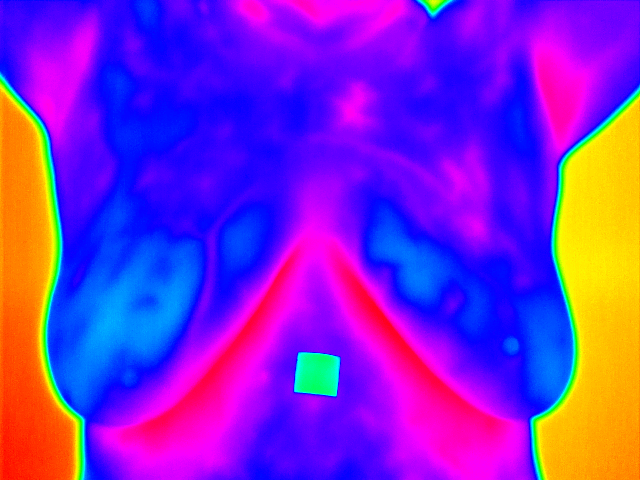
\includegraphics[width=\textwidth]{./figures_ppt/temperature_map.png}
        \caption{\label{fig:label} Temperature Map of Patient obtained
        from FLIR FLIR SC620}
      \end{figure}


    \end{column}
  \end{columns}
\end{frame}

\subsection{Dynamic Protocol}


\begin{frame}
  \frametitle{UFF's Dynamic Infrared Thermography Protocol}
  \begin{columns}
    \begin{column}{.5\textwidth}
      \begin{itemize}
      \item Applies a thermal stress to patient.
      \item Highlights vascular behavior.
      \item Captures an image every 15 seconds in 5 minutes
      \item Total sequence of 20 images.
      \item Accurate interpretation is challenged by non-specificity
        of thermal anomalies.
      \end{itemize}
    \end{column}

    \begin{column}{.5\textwidth}
      \begin{figure}[ht]
        \centering
        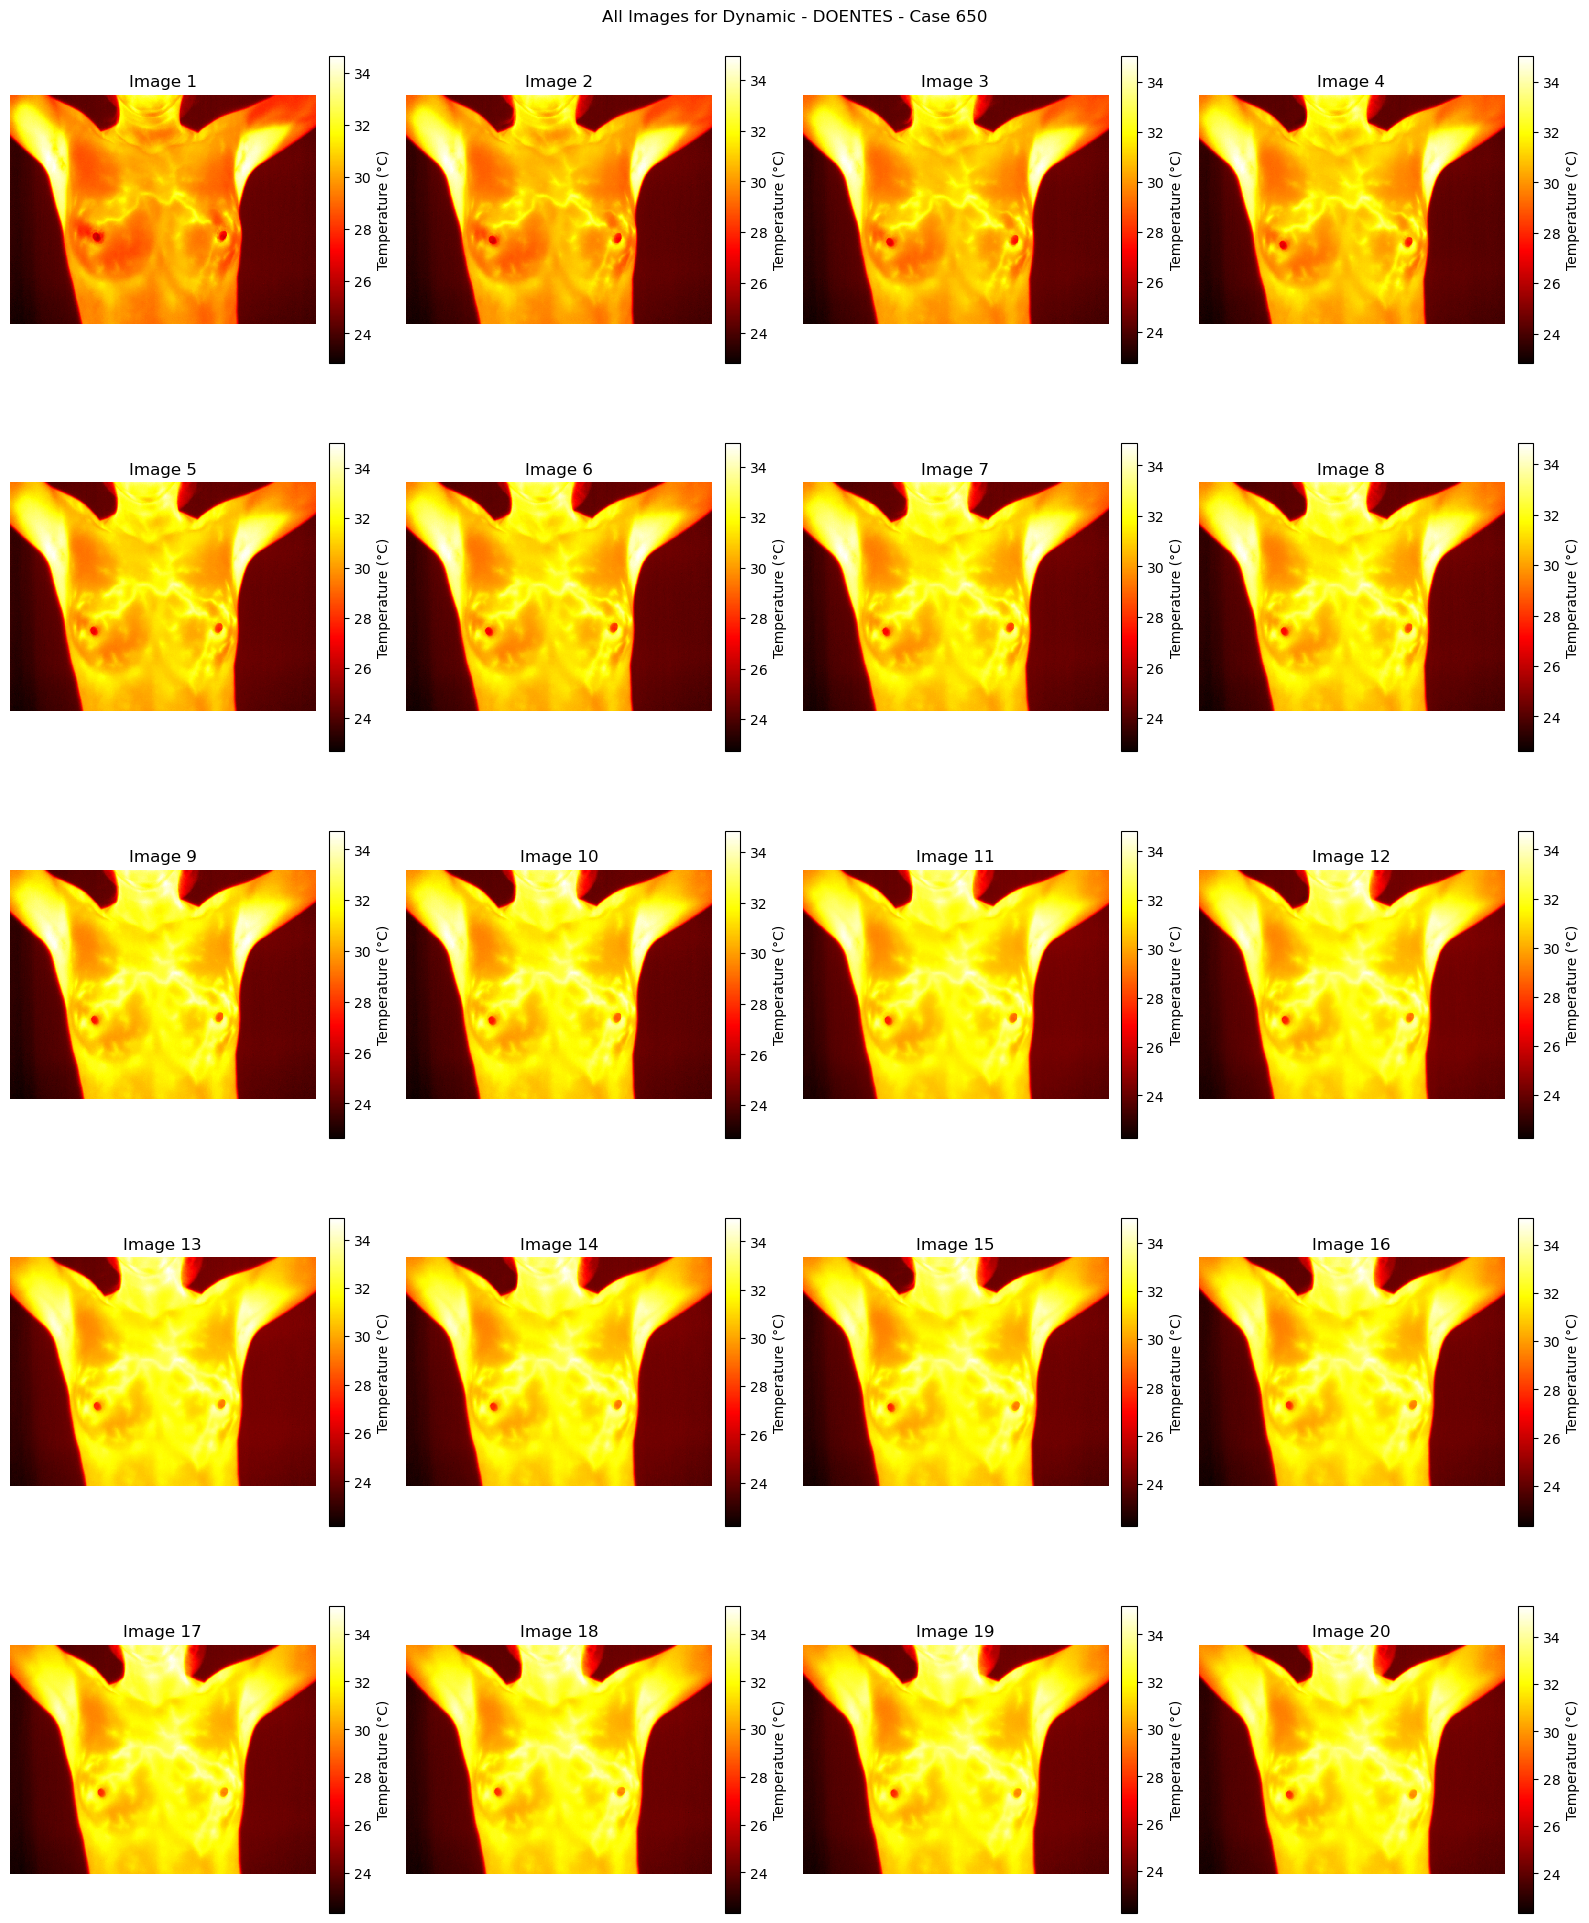
\includegraphics[width=\textwidth, height=.6\textheight]{./figures_ppt/Case650Cancer.png}
        \caption{\label{fig:label}Sequence of Thermal Maps of Patient
          650 with Cancer in UFF's Dataset }
      \end{figure}


    \end{column}
  \end{columns}
\end{frame}

\subsection{Contribution}


% --- SLIDE 4: THE CORE PROBLEM ---
\begin{frame}
  \frametitle{Paper Contribution}
\begin{enumerate}
\item Extend \ac{ViT}-based approaches to \ac{DIT} protocol.
\item Evaluate \ac{FT} of pre-trained \ac{ViTs}.
\item Conduct Experiments on thermal maps as well as \ac{IR} images.
\item \ac{FT} of a \ac{ViViT} to classify thermal images under the
  \ac{DIT} protocol ($\mathrm{AUC} = 0.9350 \pm 0.0094$),
  outperforming 3D \ac{CNNs} approaches.
\item Spatial only \ac{ViT} achieve similar performance to \ac{ViViT}.
\end{enumerate}
\end{frame}

\subsection{Research Questions}


% --- SLIDE 5: RESEARCH QUESTIONS ---
\begin{frame}
  \frametitle{Key Research Questions}
  \begin{itemize}
    \itemsep 1em
    \item \textbf{RQ1:} Do Vision Transformers (ViTs) outperform CNNs due to superior global context modeling?
    \pause
    \item \textbf{RQ2:} Does \ac{FT} improve accuracy compared to training from randomly initialized weights?
    \pause
    \item \textbf{RQ3:} Does combining pre-trained \ac{ViT} models
      with the \ac{DIT} protocol enhance performance?
  \end{itemize}
\end{frame}

% ===================================
% SECTION 2: METHODOLOGY
% ===================================
\section{Methodology}

% --- SLIDE 6: METHODOLOGY DETAILS ---
\begin{frame}
  \frametitle{Methodology Overview}
\begin{columns}
  \begin{column}{.5\textwidth}
  \begin{itemize}
\item \textbf{Dataset:} DMR-IR
  \begin{itemize}
  \item Temperature Maps $\mathbb{D}_{\mathrm{TM}}$
  \item Infrared RGB Images $\mathbb{D}_{\mathrm{IR}}$
  \end{itemize}
        \item \textbf{Analysis Unit:} Patient-level
        \item \textbf{Task:} Binary Classification (Benign vs. Malignant)
        \item \textbf{Input Data:} Sequences of 20 \ac{IR} Images
        \item \textbf{Preprocessing:} Resize to 224x224
        \item \textbf{Validation:}
        \begin{itemize}
            \item 10-Fold Cross-Validation
            \item 10\% Stratified Hold-Out Test Set (15 patients)
        \end{itemize}
      \end{itemize}    
  \end{column}

  \begin{column}{.5\textwidth}
\begin{enumerate}
\item Problem Formulation
\item Data Organization
\item Preprocessing
\item Data Partitioning
\item Model Design
\item Model Training
\item Model Evaluation
\end{enumerate}
  \end{column}
\end{columns}

\end{frame}

\subsection{Dataset Characteristics}


\begin{frame}
  \frametitle{Dataset Characteristics}
  \begin{table}[h]
  \centering
  \scriptsize
\caption{DMR-IR dataset characteristics}
\label{tab:dataset_comparison}
\begin{tabular}{lcc}
% \hline
\textbf{Feature} & $\mathbb{D}_{\mathrm{TM}}$ & $\mathbb{D}_{\mathrm{IR}}$ \\
  \hline
  Type & Temperature Map & Infrared RGB Image \\
  \hline
Matrix size & $640 \times 480$ & $640 \times 480$ \\
  Channels & 1  & 3  \\
  Number type & float(temperature) & integer(pixel) \\ 
\hline
Total patients & 55 & 149 \\
- With cancer & 36 & 87 \\
- Without cancer & 19 & 62 \\
\hline
Frames per patient & 20 & 20 \\
Total images & \numprint{1100} & \numprint{2980} \\
\hline
Training set patients & 46 & 134 \\
Test set patients & 9 & 15 \\
\hline
\end{tabular}
\end{table}
\end{frame}

% --- SLIDE 7: MODELS EVALUATED ---

\subsection{Deep Learning Models}


\begin{frame}
  \frametitle{Models Evaluated}
\begin{itemize}
\item \textbf{Time Distributed Layer Model (TDL+CNN+LSTM):}
  \begin{itemize}
  \item shares weights across all frames.
  \item applies a given layer to every frame.
  \item combines CNN and LSTM or GRU units
  \end{itemize}
\item \textbf{Modified Vision Transformer:} spatial architecture with
  attention mechanism.
\item \textbf{Video Transformer:} CNN free architecture that
  extends self-attention to space-time.
\end{itemize}
\end{frame}

\begin{frame}
  \frametitle{TDL+CNN+LSTM}
  \begin{figure}[ht]
    \centering
    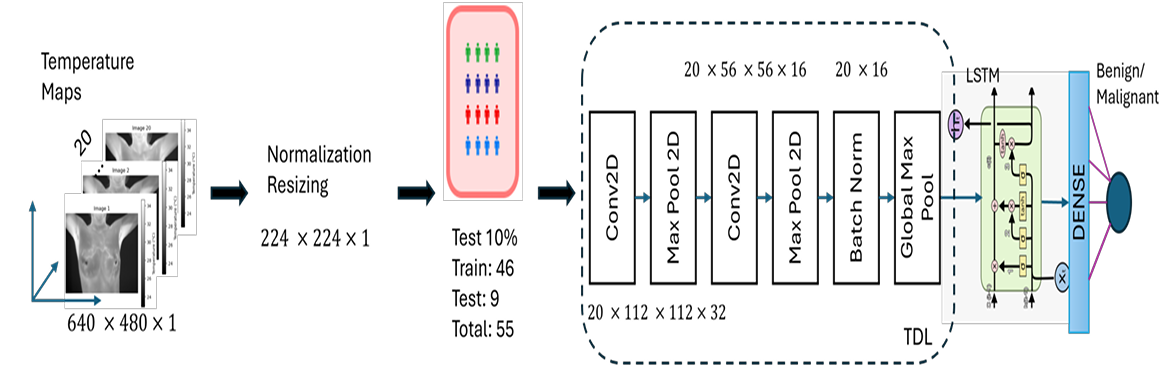
\includegraphics[width=\textwidth]{./figures_ppt/tdl.png}
    \caption{\label{fig:label} Model combining CNN and LSTM (7$\mathrm{K}$ parameters)}
  \end{figure}

  
\end{frame}
\begin{frame}
  \frametitle{Vision Transformer Models}
  \begin{figure}[ht]
    \centering
    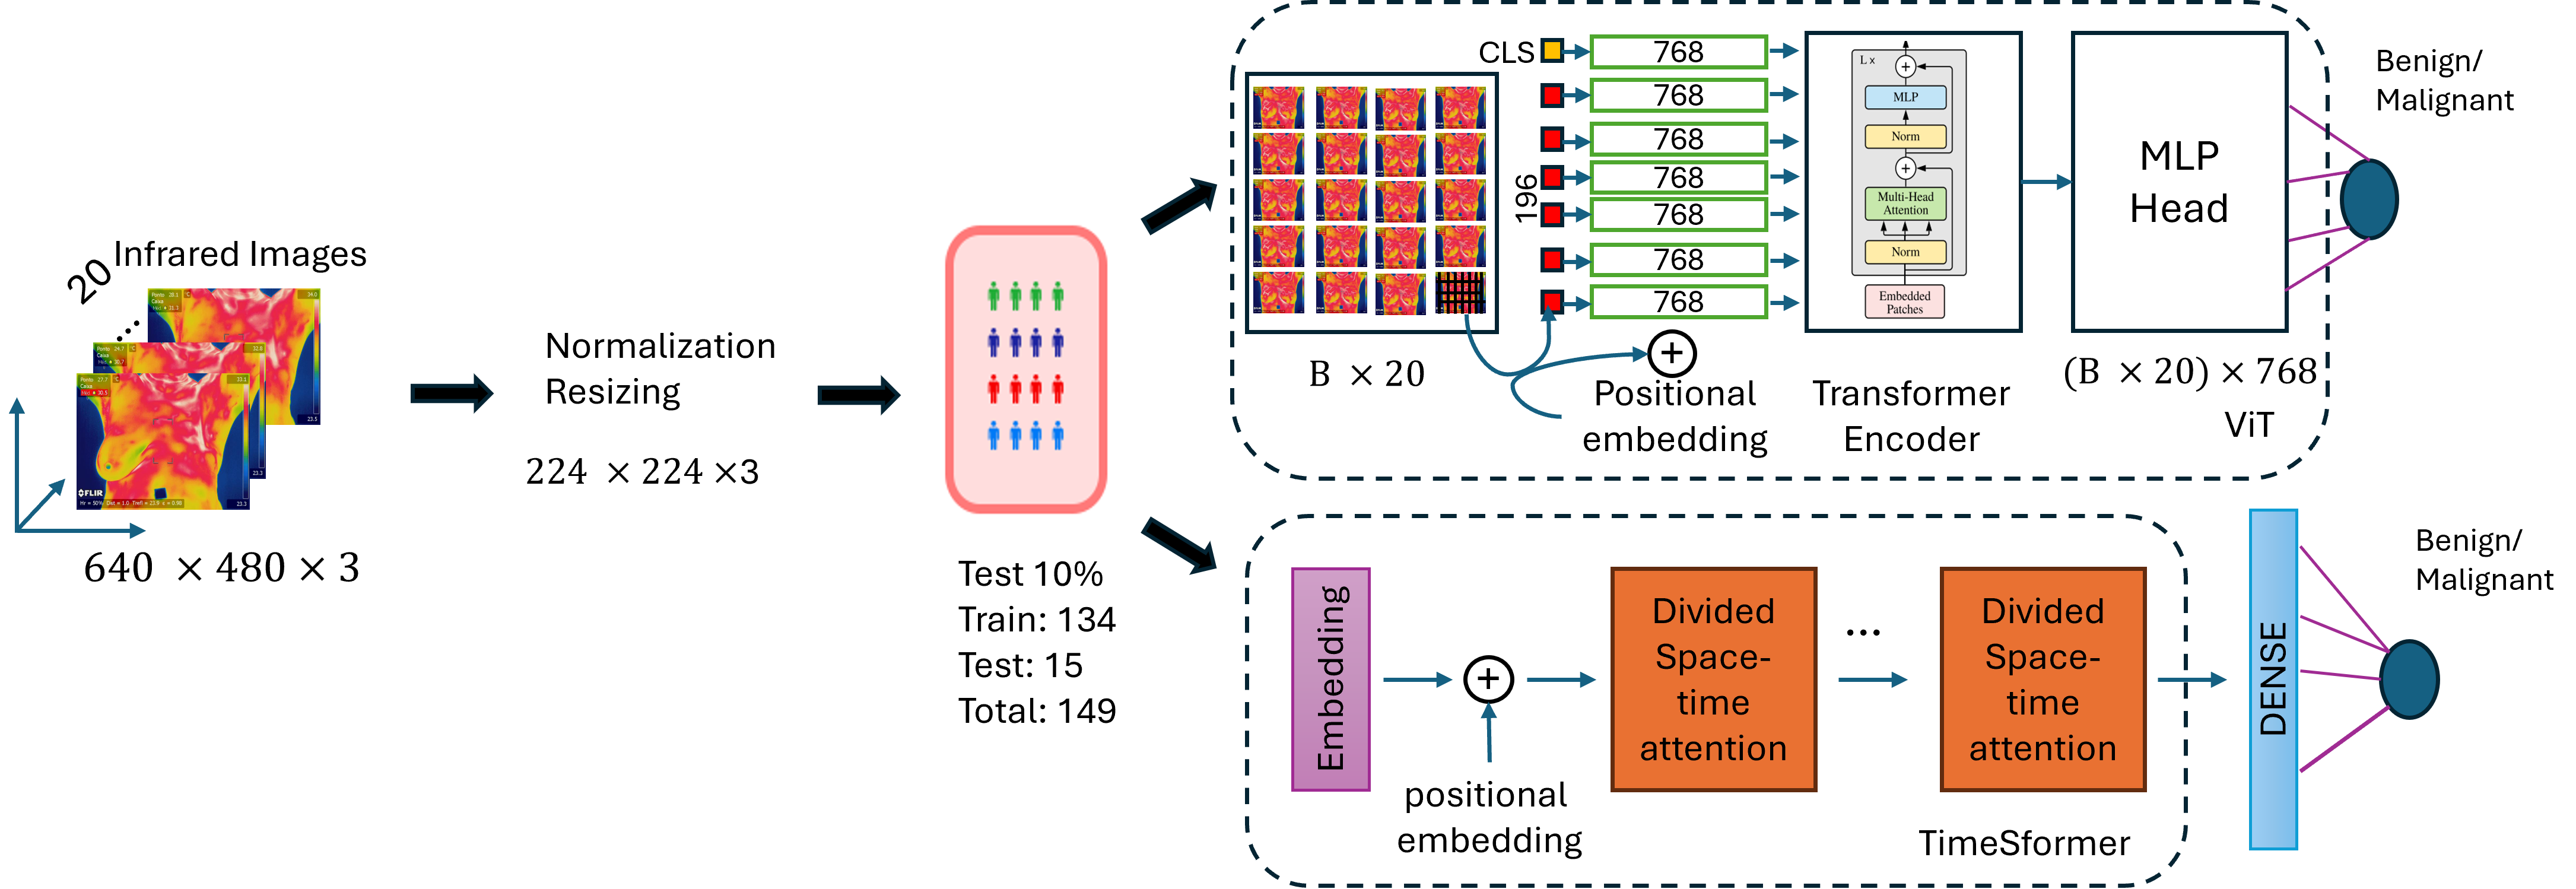
\includegraphics[width=\textwidth]{./figures_ppt/vitarch.png}
    \caption{\label{fig:label}Modified ViT ($\approx 86 \times 10^6$) loads the 20 Frames whereas
    ViViT ($\approx 121 \times 10^6$) processes 8 frames sequence in time}
  \end{figure}

\end{frame}

\subsection{Experimental Procedure}


\begin{frame}
  \frametitle{Experimental Set Up}
  \begin{figure}[ht]
    \centering
    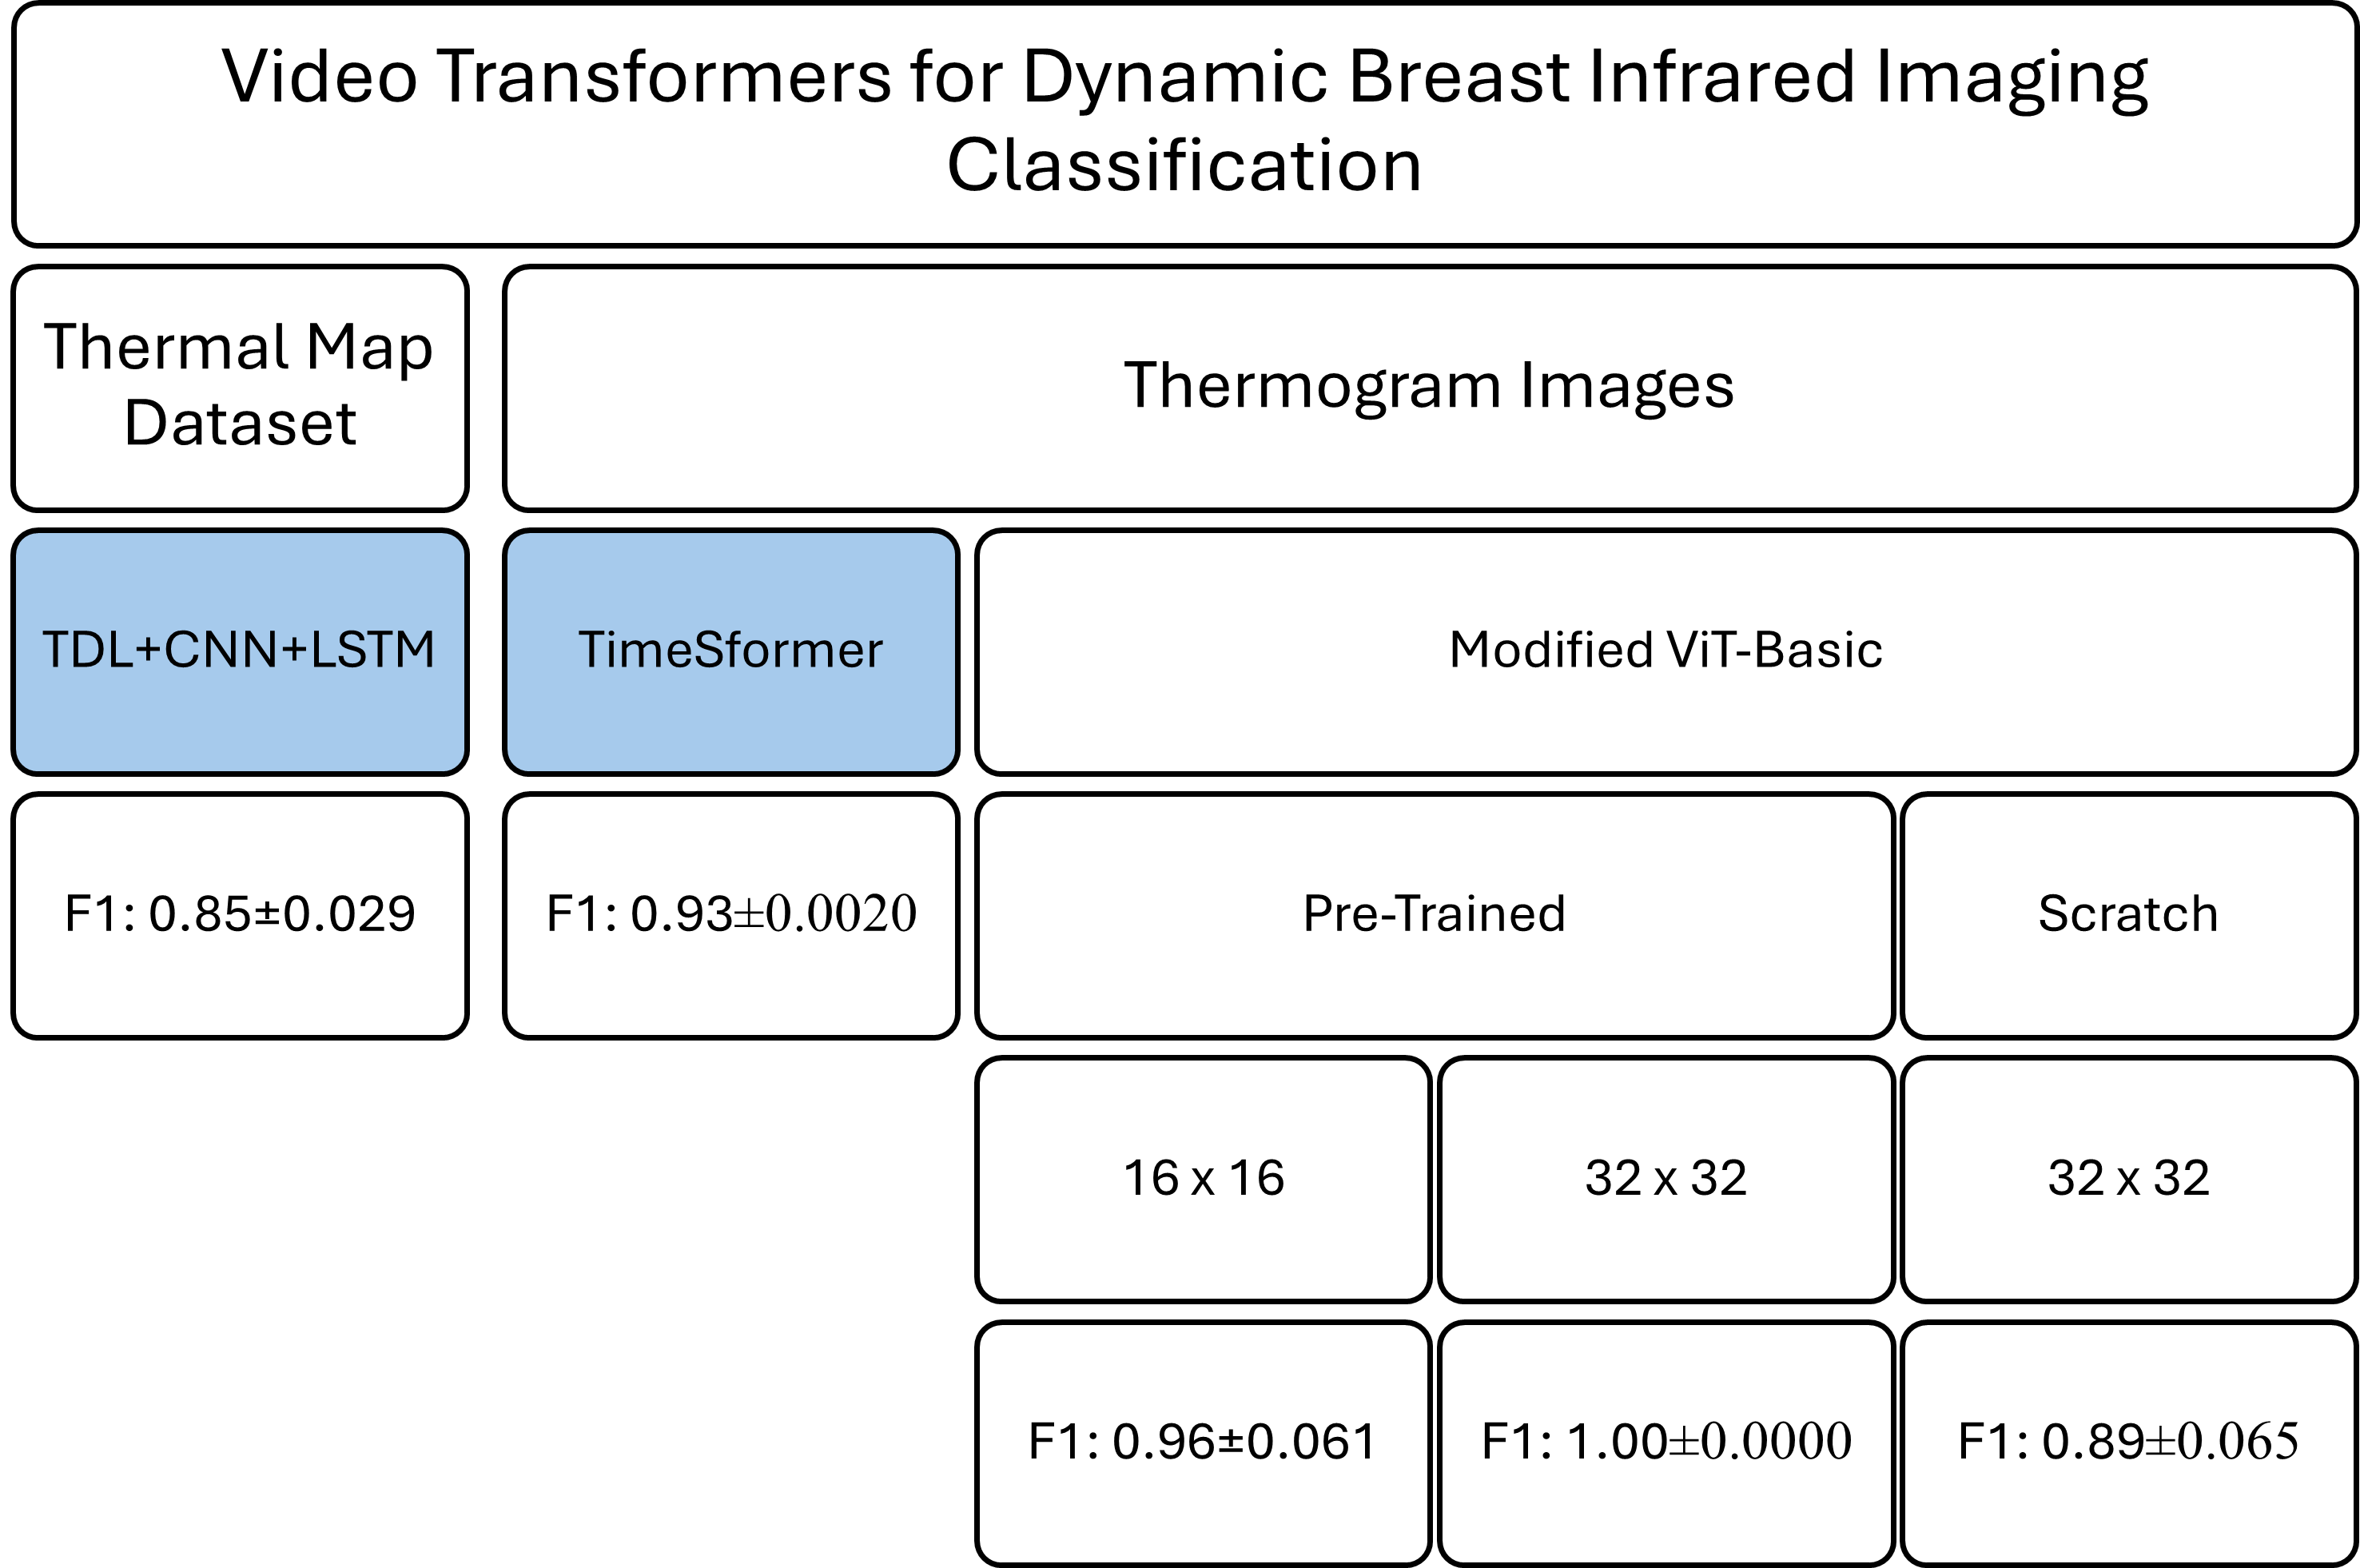
\includegraphics[width=\textwidth, height=.7\textheight]{../figures/experimentalMethodologyGuide.png}
    \caption{\label{fig:label} Guide for experimental procedure with
      results in F1-score}
  \end{figure}

\end{frame}
% ===================================
% SECTION 3: RESULTS
% ===================================
\section{Results}

\begin{frame}
  \frametitle{Performance of Different Models}
  \begin{table}[h]
  \centering
  \scriptsize
  \caption{Performance comparison of different models on \ac{DIT} data}
  \label{tab:results}
  \begin{tabularx}{\textwidth}{lXlll}
    \hline
    \textbf{Dataset} & \textbf{Model} & \textbf{Metric} & \textbf{Cross-Val (Mean $\pm$ Std)} & \textbf{Test Set} \\
    \hline
    \multirow{2}{*}{$\mathbb{D}_{\mathrm{TM}}$} & \multirow{2}{*}{TDL+CNN+LSTM} & F1-score & $0.8585 \pm 0.0296$ ($k=3$) & - \\
     & & AUC & - & - \\
    \hline
    \multirow{12}{*}{$\mathbb{D}_{\mathrm{IR}}$} & \multirow{3}{*}{ViT (16$\times$16) pre-trained} & F1-score & $0.9644 \pm 0.0458$ & - \\
     & & Accuracy & $0.9538 \pm 0.0615$ & 0.87 \\
     & & AUC & - & - \\
    \cline{2-5}
     & \multirow{3}{*}{ViT (32$\times$32) pre-trained} & F1-score & $1.0000 \pm 0.0000$ & 0.9412 \\
     & & Accuracy & $1.0000 \pm 0.0000$ & 0.9333 \\
     & & AUC & $1.0000 \pm 0.0000$ & 0.9444 \\
    \cline{2-5}
     & \multirow{3}{*}{ViT (32$\times$32) scratch} & F1-score & $0.9101 \pm 0.0665$ & 0.8889 \\
     & & Accuracy & $0.8939 \pm 0.0652$ & 0.8667 \\
     & & AUC & $0.8866 \pm 0.0595$ & 0.8611 \\
    \cline{2-5}
     & \multirow{3}{*}{ViViT} & F1-score & $0.9339 \pm 0.0020$ & 0.9412 \\
     & & Accuracy & $0.9231 \pm 0.0000$ & 0.9333 \\
     & & AUC & $0.9350 \pm 0.0094$ & 0.9444 \\
    \hline
  \end{tabularx}
\end{table}
\end{frame}
% --- SLIDE 8: KEY RESULT (BAR CHART) ---
\begin{frame}
  \frametitle{Key Result: ViViT vs. State-of-the-Art}
  \vspace{1em}
  \begin{itemize}
    \item \textbf{Baffa et al. \cite{DeMatheus2023} (3D-CNN):}
      \textcolor{structure}{\rule{0.9351\linewidth}{12pt}} \hspace{0.5em} 93.51\%
    \item \textbf{Our Work (ViViT TimeSformer):}
      \textcolor{myteal}{\rule{0.9444\linewidth}{12pt}} \hspace{0.5em} \textbf{94.44\%}
  \end{itemize}

  \vspace{1em}
  \begin{alertblock}{New State-of-the-Art}
    Our pre-trained Video Transformer (ViViT) achieved a new state-of-the-art AUC of \textbf{0.9444} on the hold-out test set, surpassing the previous 3D-CNN benchmark.
  \end{alertblock}
\end{frame}

% --- SLIDE 9: DETAILED TABLE ---
% \begin{frame}
%   \frametitle{Detailed Model Comparison (Hold-Out Test Set)}
%   \begin{table}
%     \centering
%     \small % Make text smaller to fit
%     \begin{tabular}{lllc}
%       \toprule
%       \textbf{Model} & \textbf{Pre-Trained} & \textbf{Model Type} & \textbf{Test Set AUC} \\
%       \midrule
%       TDL+CNN+LSTM & No & Spatio-Temporal (TM) & 0.8700 \\
%       ViT (32x32) & No (Scratch) & Spatial-Only & 0.8611 \\
%       ViT (16x16) & Yes (ImageNet) & Spatial-Only & 0.9333 \\
%       \midrule
%       ViT (32x32) & \textbf{Yes (ImageNet)} & \textbf{Spatial-Only} & \textbf{0.9444} \\
%       \textbf{ViViT (TimeSformer)} & \textbf{Yes (Kinetics-400)} & \textbf{Spatio-Temporal} & \textbf{0.9444} \\
%       \bottomrule
%     \end{tabular}
%     \caption{Performance on the 10\% hold-out test set (15 patients).}
%   \end{table}
% \end{frame}

\begin{frame}
  \frametitle{Comparison with Related Works}
  \begin{table}[htbp]
  \centering
  \scriptsize
\caption{Comparison of studies on breast thermography classification}
\label{tab:study_comparison}
\begin{tabularx}{\textwidth}{l *{9}{>{\centering\arraybackslash}X}}
\toprule
\textbf{Study} & \textbf{Model} & \textbf{Protocol} & \textbf{Pre-trained} & \textbf{Dataset} & \textbf{Analysis Unit} & \textbf{Total Subjects} & \textbf{Cross Validation} & \textbf{Test Set} & \textbf{AUC} \\
\midrule
Garia et al~\cite{Garia2023} & ViT & SIT & No & DMR-IR & Images & 950 & - & 10\% & 0.9570 \\
Baffa et al~\cite{DeMatheus2023} & 3D-CNN & DIT & No & DMR-IR & Patient & 149 & K=10 & - & 0.9351 \\
Our work & ViViT & DIT & Yes & DMR-IR & Patient & 149 & K=10 & 10\% & \textbf{0.9444} \\
\bottomrule
\end{tabularx}
\end{table}
\end{frame}

\subsection{Discussion}


% --- SLIDE 10: DISCUSSION ---
\begin{frame}[allowframebreaks]
  \frametitle{Discussion \& Key Findings}
\begin{itemize}
\item In $K=10$ cross validation our TimeSformer achieves similar
  performance wrt. \cite{DeMatheus2023} but with improved stability.
\item Different to \cite{DeMatheus2023}, our approach uses a spatial
  resolution of $224 \times 224$ instead of $32 \times 32$.
\item The approach does not require pre-stage segmenting breast
  region.
\item There is a risk for overfitting due to limited dataset size and
  large architectures.
\item \ac{FT} and data augmentation help to mitigate overfitting.

\end{itemize}
\newpage
\begin{itemize}
\item \textit{Do \ac{ViTs} outperfom \ac{CNNs}-based approaches in
  \ac{TG} \ac{BC} classification?} Yes, this was demonstrated in
\cite{Garia2023} and this work.
\item \textit{What is better \ac{FT} or from scratch?} Our results
  differ from those in \cite{Garia2023} and show that fine-tuned
  models achieve a better performance.
\item \textit{Does combining \ac{ViTs} and \ac{DIT} enhance
    performance?} Further research is needed. Our results show that a
  traditional spatial based \ac{ViT} achieve a similar performance to
  that of the \ac{ViViT}:
  \begin{enumerate}
  \item TimeSformer uses 8 frames by default
  \item Given the result in \cite{Garia2023} where \ac{SIT} is used,
    further research is needed on the impact of \ac{DIT} in results.
  \item \ac{TG} is susceptible to other sources of temperature change
    in the patient which may need to be acknowledged.
  \end{enumerate}

\end{itemize}
\end{frame}
% ===================================
% SECTION 4: CONCLUSION
% ===================================
\section{Conclusion}

% --- SLIDE 11: CONCLUSION ---
\begin{frame}
  \frametitle{Conclusion \& Future Work}
  \begin{itemize}
    \item We present the first study to apply \textbf{Video Vision Transformers (ViViT)} to the DIT protocol for breast cancer classification.
    \item Our model achieves \textbf{state-of-the-art performance ($0.9444$ AUC)} on the DIT patient-level task.
    \item We demonstrate that \textbf{fine-tuning pre-trained models}
      is necessary to mitigate overfitting due to limited dataset
      size.
    \item Performance of pre-trained models is better than that of
      \ac{TDL} model on temperature Maps.
    \item Pre-trained models work better when using \ac{IR} images
      than temperature maps.
    \item \textbf{Future Work:} Further research is needed to
      investigate the true value of temporal dynamics in DIT versus
      spatial-only modeling and texture based approaches.
  \end{itemize}
\end{frame}

% --- SLIDE 12: Q&A ---
\begin{frame}
  \frametitle{} % No title
  \centering
  \Huge
  Thank You
  \vspace{1em}
  \Large
  Questions?
  \vfill
  \small
  Lenin G. Falconi: lenin.falconi@epn.edu.ec \\
\end{frame}
% Bibliography
\begin{frame}[allowframebreaks]
    \frametitle{References}
    % \nocite{*} % This command will include all entries from your .bib file
    \printbibliography
\end{frame}
\end{document}


%%% Local Variables:
%%% mode: LaTeX
%%% TeX-master: t
%%% End:
